\documentclass[../main.tex]{subfiles}
\graphicspath{
    {"../img/"}
    {"img/"}
}

\begin{document}
    \subsection{Przypomnienie}
    \begin{figure}[h]
        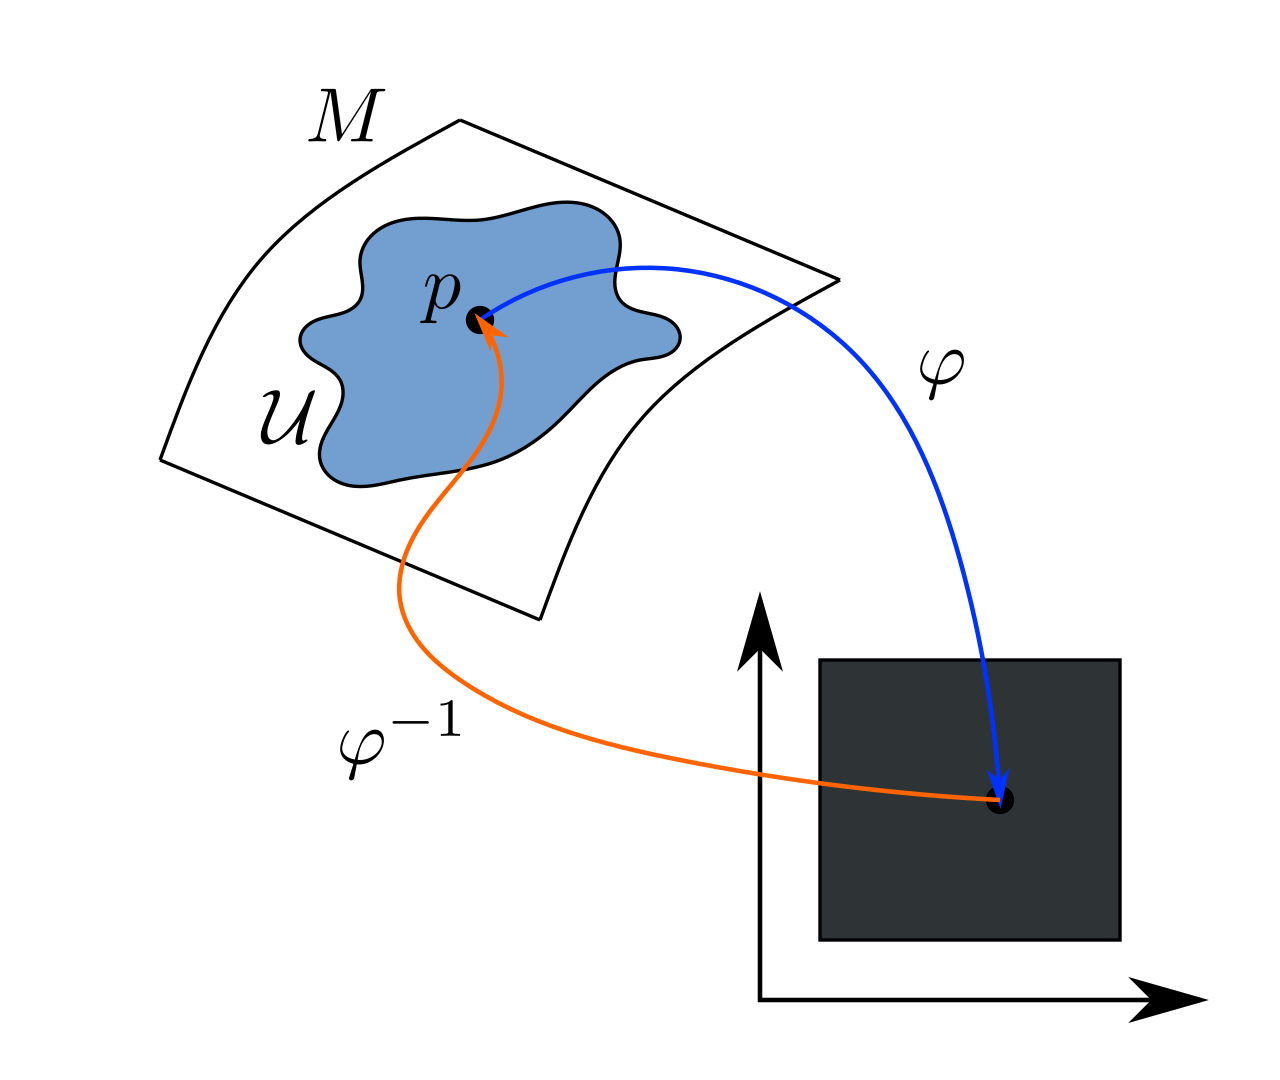
\includegraphics[width=0.4\textwidth]{fig1-1}
        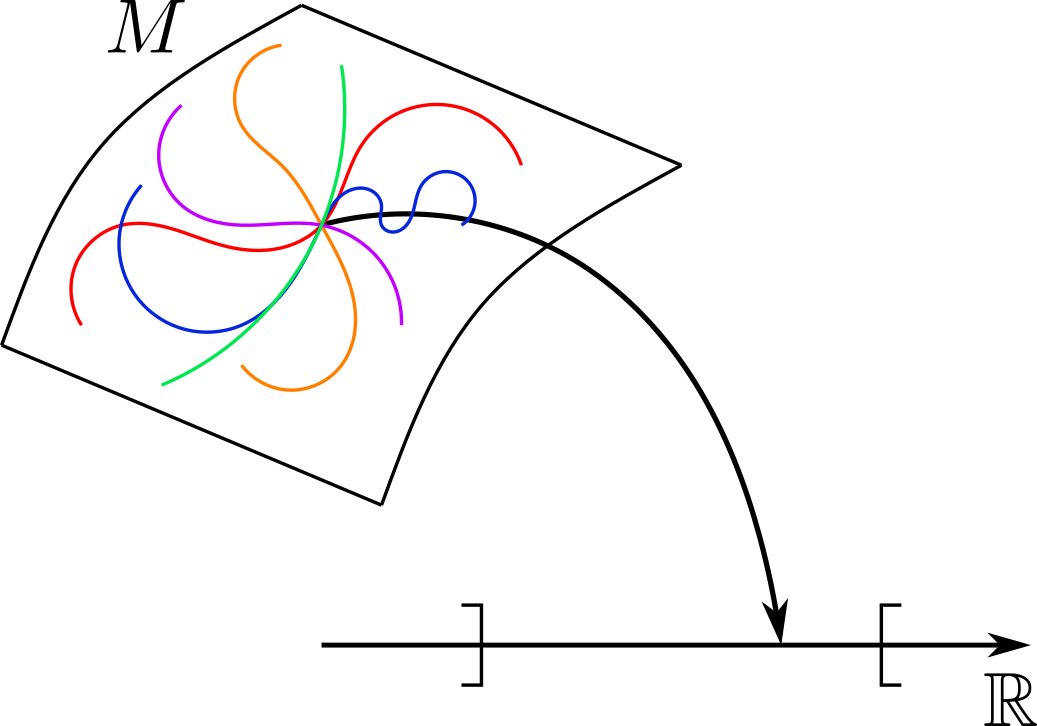
\includegraphics[width=0.4\textwidth]{fig1-2}
        \caption{Przypomnienie}
        \label{fig:fig1-1}
    \end{figure}
    Niech $\alpha_1, \alpha_2, \ldots, \alpha_k \in \Lambda^1(M)$, $v_1, v_2, \ldots, v_k \in T_pM$, to wtedy
    \[
        \left<\alpha_1\land \alpha_2\land \ldots\alpha_k, v_1, v_2, \ldots, v_k \right> = \left| \begin{bmatrix} \alpha_1(v_1) & \ldots & \alpha_k\\ \vdots & \ddots & \vdots\\ \alpha_1(v_k) & \ldots & \alpha_k(v_k) \end{bmatrix} \right|
    .\]
    \begin{figure}[h]
        \centering
        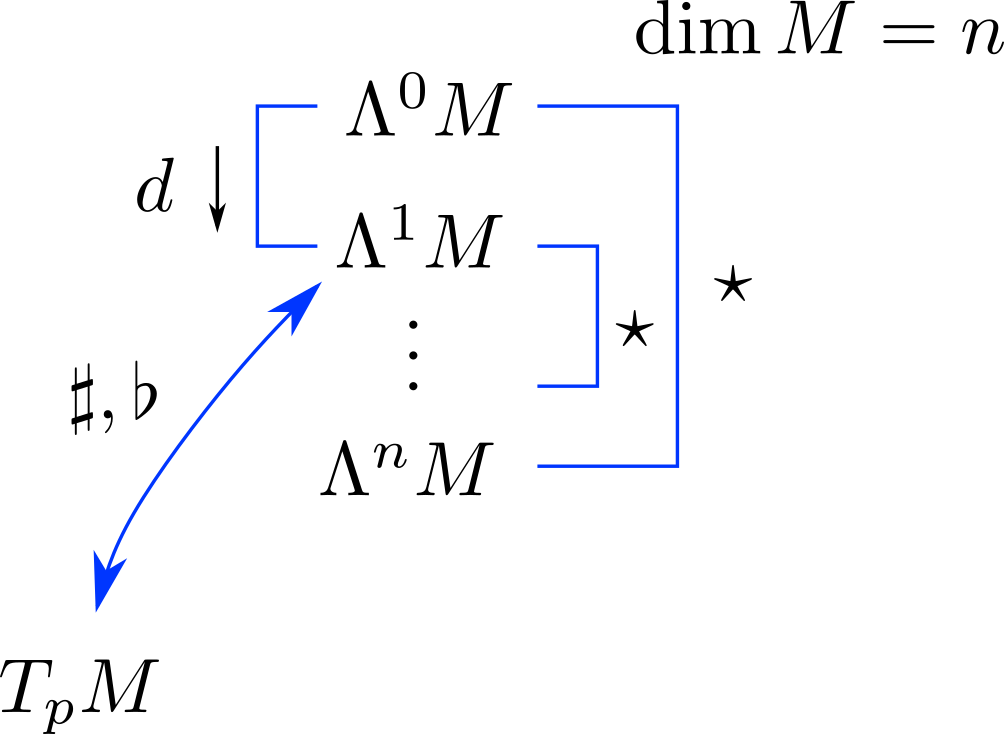
\includegraphics[width=0.5\textwidth]{fig1-3}
        \caption{Przypomnienie c.d.}
        \label{fig:fig1-3}
    \end{figure}
    \[
        \left< v | w \right> = [v]^T [g_{ij}] \begin{bmatrix} \\w \\ \\ \end{bmatrix}
    .\]
\[
    A = A^1 \frac{\partial }{\partial x^1} + \ldots + A^n \frac{\partial }{\partial x^n}
.\]
\[
A^\sharp = A^1g_{11}dx^1 + \ldots + A^ng_{nn}dx^n
,\]
(gdy $g_{ij}$ - diagonalna)
\[
    A^ig_{ij}dx^j
.\]
\subsection{To jak to było z tymi wektorami?}
Niech $A\in T_pM$,  $A = A^1 \frac{\partial }{\partial x^1} + \ldots + A^k \frac{\partial }{\partial x^k} $, $B = T_pM$, $B = B^1 \frac{\partial }{\partial x^1} + \ldots + \frac{\partial }{\partial x^k}$.\\
Jaka jest interpretacja geometryczna wielkości
\[
    \left<A^\sharp, B \right>,\quad (g_{ij}\text{ - diagonalna})
.\]
\[
A^\sharp = A^1g_{11}dx^1 + \ldots + A^kg_{kk}dx^k
.\]
\begin{align*}
    \left<A^\sharp, B \right> &= \left<A^1g_{11}dx^1 + \ldots + A^k g_{kk}dx^k, B^1 \frac{\partial }{\partial x^1} + \ldots + B^k \frac{\partial }{\partial x^k}  \right> = \\
    &=  g_{11}A^1B^1 + \ldots + g_{kk}A^kB^k = A\cdot B
.\end{align*}
Czyli gdyby $\left\Vert B \right\Vert = 1$, to $\left<A^\sharp, B \right>$ byłoby długością rzutu $A$ na kierunek $B$.\\
Niech $\dim M = 3$, $\Lambda^2M\ni A$,
\[
A = A^1 dx^2\land dx^3 + A^2dx^3\land dx^1 + A^3dx^1\land dx^2
.\]
\[
B = B^1 \frac{\partial }{\partial x^1} + B^2 \frac{\partial }{\partial x^2} + B^3 \frac{\partial }{\partial x^3},\quad C = C^1 \frac{\partial }{\partial x^1} + \ldots + C^3 \frac{\partial }{\partial x^3} \in T_pM
.\]
\begin{align*}
    \left<A, B, C \right> &= A^1 \left<dx^2\land dx^3, B, C \right> + A^2\left<dx^3\land dx^1, B, C \right> + A^3 \left<dx^1\land dx^2, B, C \right> = \\
    &= A^1 \begin{bmatrix} \left<dx^2, B \right>& \left<dx^3, B \right>\\ \left<dx^2, C \right>& \left<dx^3, C \right> \end{bmatrix} + A^2 \begin{bmatrix} \left<dx^3, B \right> & \left<dx^1, B \right> \\ \left<dx^3, C \right> & \left<dx^1, C \right> \end{bmatrix} + \\
        &+ A^3\begin{bmatrix} \left<dx^1, B \right> & \left<dx^2, B \right> \\ \left<dx^1, C \right> & \left<dx^2, C \right> \end{bmatrix}  =\\
        &= A^1\begin{bmatrix} B^2&B^3\\C^2&C^3 \end{bmatrix} + A^2\begin{bmatrix} B^3&B^1\\C^3&C^1 \end{bmatrix} + A^3\begin{bmatrix} B^1&B^2\\C^1&C^2 \end{bmatrix} =\\
            &=  A^1 \left( B^2C^3 - B^3C^2 \right) + A^2 \left( B^3C^1 - B^1C^3 \right) + A^3 \left( B^1C^2 - B^2C^1 \right) =\\
            &"=" A^1 (B\times C)_1 + A^2(B\times C)_2 + A^3(B\times C)_3 "=" A\cdot (B\times C) \\
            &= \left|\begin{bmatrix} A^1 & A^2 & A^3\\ B^1&B^2&B^3\\ C^1&C^2&C^3 \end{bmatrix}\right|
.\end{align*}
Wychodzi tak jak na (rys \ref{fig:fig1-4})\\
\begin{figure}[h]
    \centering
    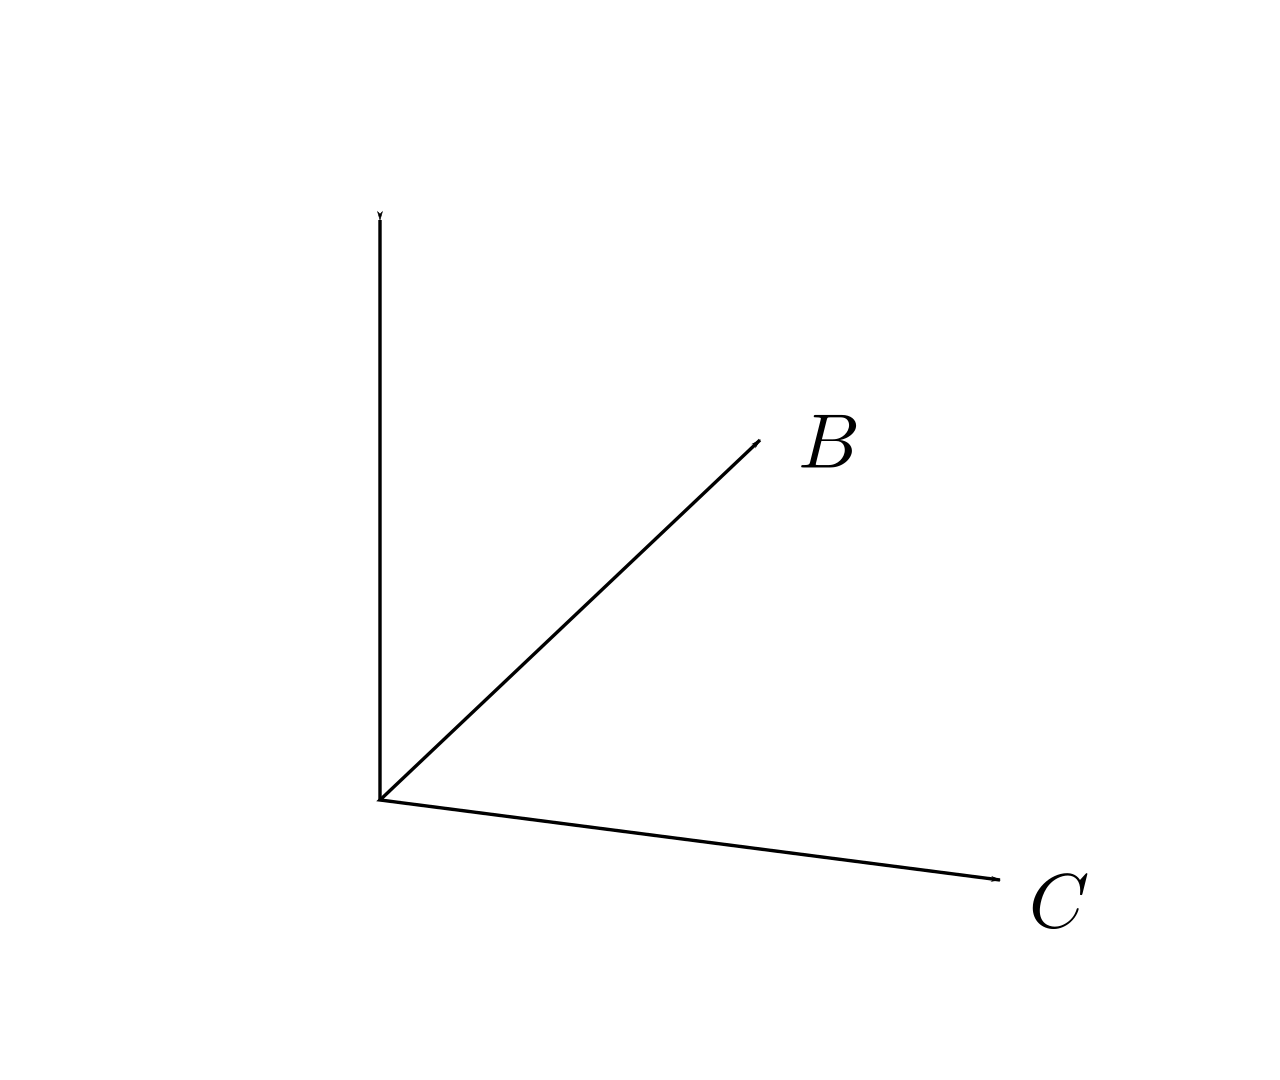
\includegraphics[width=0.3\textwidth]{fig1-4}
    \caption{Się okazuje, że wychodzi z tego coś jak iloczyn wektorowy}
    \label{fig:fig1-4}
\end{figure}
\subsection{Problem}
$\dim M = 3$, mamy
 \[
\Lambda^1M\ni F = F^1dx^1 + F^2dx^2 + F^3dx^3
\]
oraz krzywą $S$ w $\mathbb{R}^3$ (np. spiralę) (rys \ref{fig:fig1-4}). Chcemy znaleźć pracę związaną z przemieszczeniem z punktu $A$ do $B$.
\begin{enumerate}
    \item sparametryzujmy kształt $S$, np.
        \[
            S = \left\{ (x,y,z)\in\mathbb{R}^3, \begin{matrix}x = \cos(t)\\ y = \sin(t)\\ z = t \end{matrix}, t\in \left[ 0, 4\pi \right] \right\}
        .\]
\item możemy na spirali wygenerować pole wektorów stycznych. \\
    Jeżeli $p = \left.\begin{bmatrix} \cos(t)\\ \sin(t)\\ t \end{bmatrix}\right|_{t = t_0} $, to
        \[
            T_pM = \left.\left<\begin{bmatrix} -\sin(t)\\ \cos(t)\\ 1 \end{bmatrix}  \right>\right|_{t = t_0}
                .\] (rys \ref{fig:fig1-5})
        \item Niech $T_pM \ni v = -\sin(t) \frac{\partial }{\partial x} + \cos(t) \frac{\partial }{\partial y} + \frac{\partial }{\partial z}$. (rys \ref{fig:fig1-6})\\
            Możemy policzyć np.
            \begin{align*}
                \int \left<F, v \right> &= \int\limits_{0}^{4\pi} \left<F, -\sin(t)\frac{\partial }{\partial x} + \cos(t) \frac{\partial }{\partial y} + \frac{\partial }{\partial z}  \right> dt = \\
                &= \int\limits_{0}^{4\pi} \left<F, \varphi_\star\left(\frac{\partial }{\partial t} \right) \right>dt = \int\limits_0^{4\pi} \left<\varphi^\star F, \frac{\partial }{\partial t}  \right>dt
            .\end{align*}
\end{enumerate}
\begin{figure}[h]
    \centering
    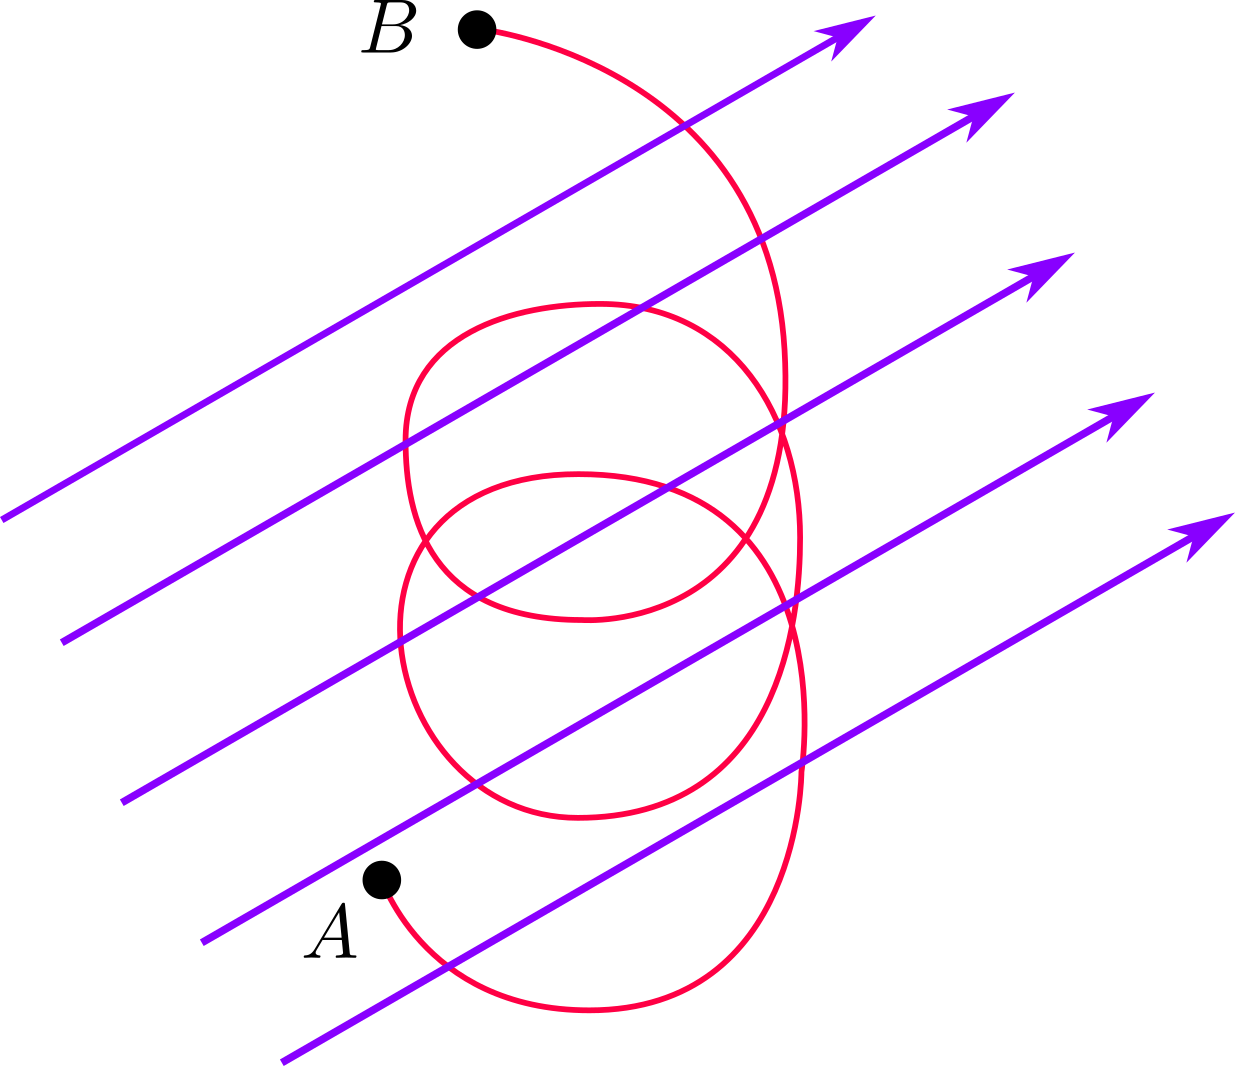
\includegraphics[width=0.4\textwidth]{fig1-5}
    \caption{Mrówka (albo koralik) na spirali + jakieś pole wektorowe (grawitacyjne albo mocny wiatrak)}
    \label{fig:fig1-5}
\end{figure}
\begin{figure}[h]
    \centering
    
\includegraphics[width=0.3\textwidth]{fig1-6}
    \caption{można jakoś to sparametryzować przez $\varphi$}
    \label{fig:fig1-6}
\end{figure}
\begin{figure}[h]
    \centering
    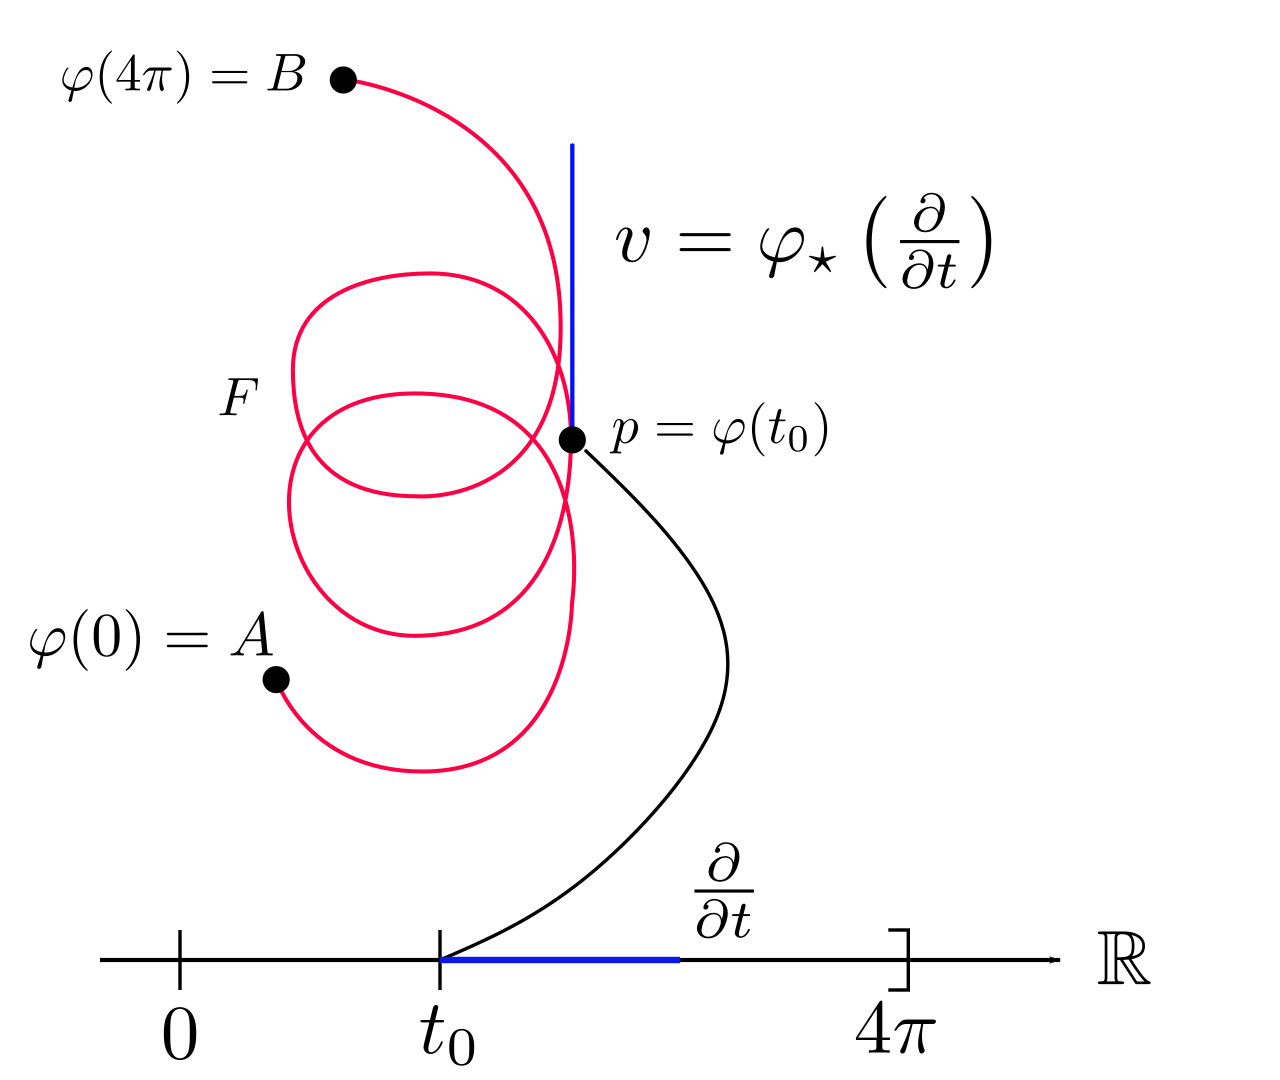
\includegraphics[width=0.6\textwidth]{fig1-7}
    \caption{}
    \label{fig:fig1-7}
\end{figure}

\pagebreak
\begin{definicja}
    Niech $M$ - rozmaitość, $L$ - krzywa na $M$, $w\in \Lambda^1M$, $\varphi: [a,b] \to M$ - parametryzacja krzywej $L$, czyli
    \[
        L = \left\{ \varphi(t), t\in [a,b] \right\}
    .\]
Całką z jednoformy po krzywej nazywamy wielkość (rys \ref{fig:fig1-7})
\[
\int\limits_a^b \left<\varphi^\star \omega, \frac{\partial }{\partial t}  \right>dt
.\]
\end{definicja}
\begin{figure}[h]
    \centering
    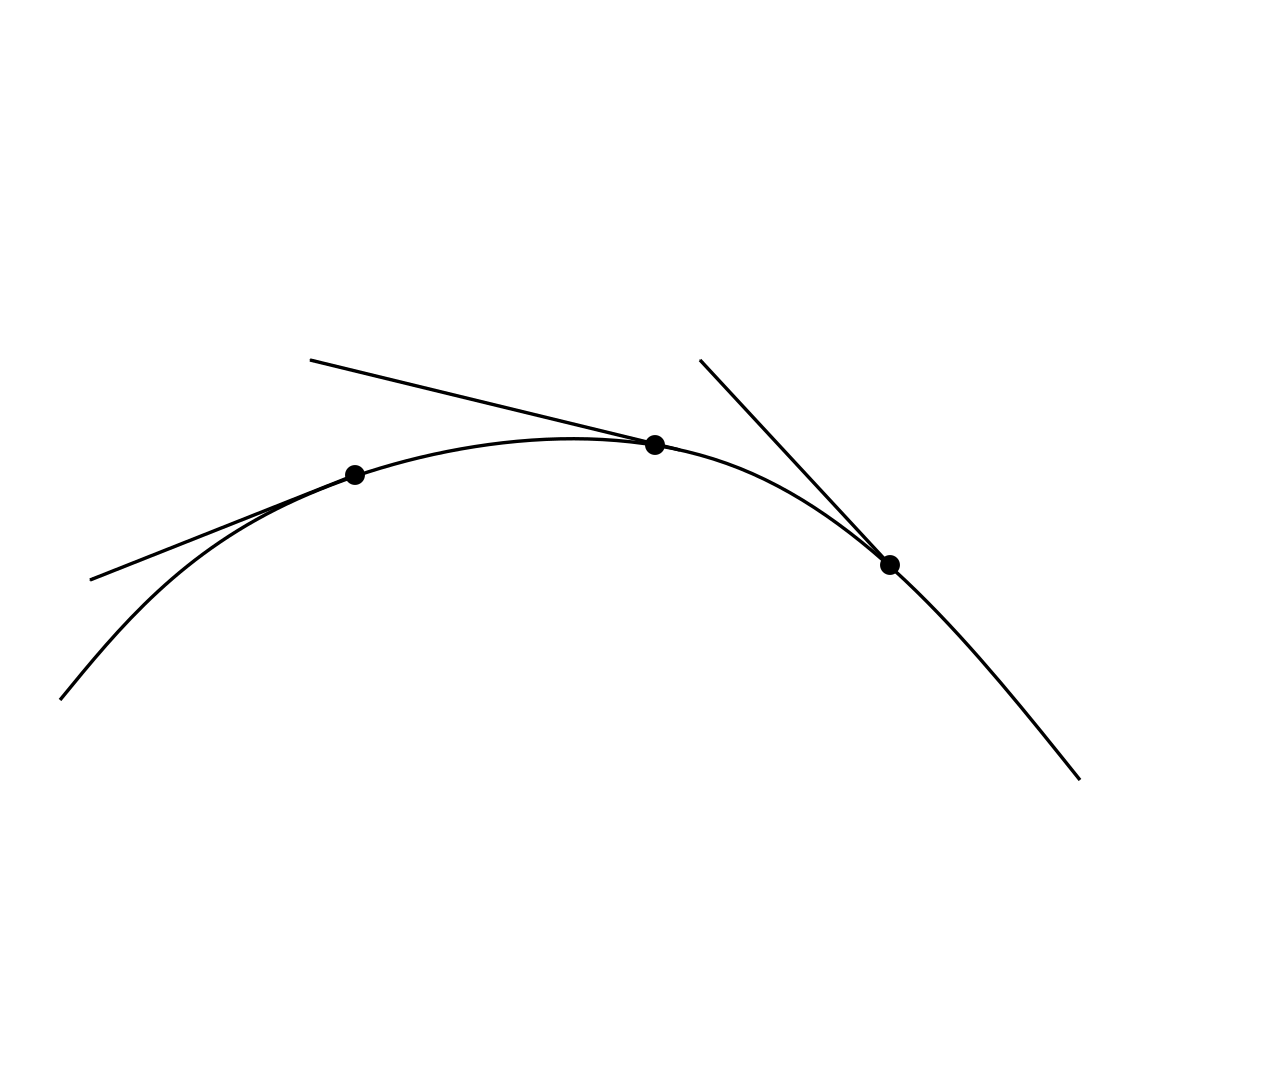
\includegraphics[width=0.5\textwidth]{fig1-8}
    \caption{Cała sztuka polega na takim kolekcjonowaniu wektorków stycznych}
    \label{fig:fig1-8}
\end{figure}
\begin{przyklad}
    niech (rys \ref{fig:fig1-8})
 \[
     C_1 = \left\{ (x,y)\in \mathbb{R}^2, \begin{bmatrix} x\\y \end{bmatrix} = \begin{bmatrix} t-1\\2t-1 \end{bmatrix}, 1\le t\le 2 \right\}
\]
i
    \[
        \omega = ydx = \left( y \frac{\partial }{\partial x}  \right)^\sharp
    .\]
Wtedy mamy $\varphi(t) = \begin{bmatrix} t-1\\2t-1 \end{bmatrix} $, $\varphi^\star \omega =\quad \left| \begin{matrix}x=t-1\\dx = dt\end{matrix}\right| = (2t-1)dt$
    \begin{align*}
        &\left<\varphi^\star \omega, \frac{\partial }{\partial t}  \right> = \left<(2t-1)dt, \frac{\partial }{\partial t}  \right> = 2t-1\\
        \int\limits_{C_1}\omega &= \int\limits_1^2\left<\varphi^\star\omega, \frac{\partial }{\partial t}  \right>dt = \int\limits_1^2 (2t-1)dt = \left[ t^2 - t \right]_1^2 =  2\\
    .\end{align*}

    \[
        C_2 = \left\{ (x,y)\in \mathbb{R}^2, \begin{bmatrix} x\\y \end{bmatrix} = \begin{bmatrix} 2-u\\5-2u \end{bmatrix}, 1\le u \le 2 \right\}, \varphi_1(u) = \begin{bmatrix} 2-u\\5-2u \end{bmatrix}
    .\]
\[
\int\limits_{C_2}\omega = \int\limits_1^2 \left<\varphi_1^\star \omega, \frac{\partial }{\partial u}  \right>du
,\]
ale $\begin{matrix}x = 2-u\\ dx = -u\end{matrix}$ i mamy
     \[
         \varphi^\star \omega = (5-2u)(-du) = (2u-5)du
    .\]
Ostatecznie
\[
    \int\limits_{C_2}\omega = \int\limits_1^2(2u-5)du = \left[ u^2 - 5u \right] _1^2 = -6+4 = -2
.\]
\end{przyklad}

\end{document}
